% Hello friend, this doc is still in the works but should eventually contain the homework questions for each of the 12 homework sets, beautifully typeset.

% bump chapter num ahead since we re-declare \appendix in main.tex
\setcounter{chapter}{1}
\chapter*{Homework Sets}
\addtocounter{chapter}{1} % Manually increment the chapter counter
\markboth{\sffamily\normalsize\bfseries Homework Sets}{} % Set the chapter header
\addcontentsline{toc}{chapter}{\textcolor{ocre}{Homework Sets}}

\section{Homework \# 1 }
\markright{\sffamily\normalsize Homework \# 1} % Set the section header
\label{sec:HW1}
\index{Homework 001@Homework \#1}

\begin{enumerate}
    \item Define relation $\sim$ on $\R$ as follows:
    \begin{align}
        \forall \ r,s \in \R, \ \ \ r\sim s \iff r-s\in \Z \nonumber
    \end{align}
    Prove that $\sim$ is an equivalence relation on $\R$. \\ \steezybreak

    \item Assume that $\sim$ is the equivalence relation on $\R$ from problem 1.
    \begin{enumerate}[label=\alph*)]
        \item Describe the set that is $cl(\pi)$, the equivalence class of pi.
        \item Into how many equivalence classes does $\sim$ break $\R$? \\ \steezybreak
        
    \end{enumerate}
    \item Use the definition of ``even" given in class to prove that the following relation $\sim$ on $\Z$ is an equivalence relation:
    \begin{align}
        \forall \ n,m \in \Z, n\sim m \iff n+m \text{ is even.}\nonumber
    \end{align}
    \item Describe the equivalence classes of $\Z$ under the relation $\sim$ in problem 3. \\ \steezybreak
    
    \item Suppose $\sigma : \R \mapsto \Z$ is the ``ceiling function": $\forall r\in \R,$ $\sigma(r)$ is the smallest integer $\geq r$. Is $\sigma$ a bijection? (Either prove it or give a counterexample). \\ \steezybreak
    
    \item Assume $\alpha, \beta,$ and $\gamma$ are mappings from a set $S$ to itself, with $\gamma$ both injective and surjective. \\ \\
    Prove: If $\alpha \circ \gamma = \beta \circ \gamma$, then $\alpha = \beta$.
\end{enumerate}
\newpage

%\thispagestyle{plain}
\section{Homework \# 2}
\markright{\sffamily\normalsize Homework \# 2} % Manually Set the section header
\label{sec:HW2}
\index{Homework 002@Homework \#2}

\begin{enumerate}
    \item Assume $a=138,000$ and $b=102,810$. Use the Euclidean Algorithm to calculate the greatest commond divisor of $a$ and $b$. \\ \steezybreak
    
    \item Same $a$ and $b$ from problem 1. Use matrices to find integers $n$ and $m$ for which
    \begin{align}
        GCD(a,b)=na+mb \nonumber
    \end{align}
    \item Assume $a,b,c\in \Z$, with $a$ relatively prime to both $b$ and $c$. Use Lemma 1.3.1 to prove that $a$ is relatively prime to the product $bc$. \\ \steezybreak

    \item Suppose $n,m,a \in \Z$, with $n$ and $m$ relatively prime. Show that if $n|a$ and $m|a$, then $nm|a$. \\ \steezybreak
    
    \item Consider $\Z$ under the equivalence relation $\equiv \mod n$ and assume $a\in \Z$. Prove that if $a$ is relatively prime to $n$, then \textit{every} element in $[a]$ is relatively prime to $n$. \\ \steezybreak
    
    \item Suppose $G$ is a group of order $4$; Say $G=\{e,a,b,c\}$ under an (unspecified) operation, with identity element $e$. Prove that $G$ must be abelian by displaying all possible Cayley tables for $G$.
\end{enumerate}
\newpage

\section{Homework \# 3}
\markright{\sffamily\normalsize Homework \# 3} % manually set the section header
\label{sec:HW3}
\index{Homework 003@Homework \#3}

In problem \#6 of this homework you will begin working with your own personal group, you will investigate this group for the remainder of the course. Choose one from the list below this homework set (See next page). \\ \steezybreak

\begin{enumerate}
    \item Assume that $G$ is a group of order $n$. Prove that the number of $e$'s off the main diagonal in the Cayley table for $G$ must be even. \\ \steezybreak
    
    \item Use the result from problem 1 to prove this: Every group of even order has at least one element of order $2$. \\ \steezybreak
    
    \item Define
    \begin{align}
        H&= \{2\times 2 \text{ invertible matrices with entries in }\R\text{ whose columns sum to }1\} \nonumber \\
        &= \left \{\begin{pmatrix}
            r&s\\t&u
        \end{pmatrix}\big | \ r,s,t,u \in \R, ru-st\neq 0, r+t=1, s+u=1 \right \} \nonumber
    \end{align}
    Prove that $H<GL_2(\R)$ \\ \steezybreak

    \item Assume that $G$ is a group and suppose that every nontrivial element of $G$ has order $2$. Prove that $G$ is abelian. \\ \steezybreak
    
    \item Assume that $G$ is a group and suppose that $\forall \ x,y \in G$, $\ \ x^2y^2=(xy)^2$. Prove that $G$ is abelian. \\ \steezybreak
    
    \item Construct the Cayley table for your personal group \footnote{Recall the procedure from Example \ref{ex:ConstructingFromGenerators} for constructing a group from generators $a,\ b,\ c,\ldots$.}, taking care not to use different names for the same element. Keep a minimal$^{(*)}$ list of the relations you discover as you fill in the table. Finally, note the order of your group and whether or not it is abelian. \\ \\ \\ $(*)$ ``minimal" means ``as short as possible," so leave out any relation that can be deduced from the others in your list.
\end{enumerate}
\newpage
% Personal Groups go here:
\subsection{Personal Groups (CHOOOSE ONE)}
\begin{enumerate}
    \setlength{\itemsep}{5pt} % Adjusts spacing between items
    \item[\#1)] \( a = \begin{bmatrix} -1 & -1 & 0 \\ 1 & 0 & 0 \\ 0 & 0 & -1 \end{bmatrix}, \quad
                 b = \begin{bmatrix} 0 & 1 & 0 \\ 1 & 0 & 0 \\ 0 & 0 & 1 \end{bmatrix} \)
                 \quad multiply
    \item[\#2)] \( a = \begin{bmatrix} -1 & 0 & 0 \\ 0 & 1 & 0 \\ 0 & 0 & 1 \end{bmatrix}, \quad
                 b = \begin{bmatrix} 1 & 0 & 0 \\ 0 & -1 & 0 \\ 0 & 0 & 1 \end{bmatrix}, \quad
                 c = \begin{bmatrix} 1 & 0 & 0 \\ 0 & 1 & 0 \\ 0 & 0 & -1 \end{bmatrix} \)
                 \quad multiply
    \item[\#3)] \( a = \begin{bmatrix} 4 & 2 \\ 0 & 1 \end{bmatrix}, \quad
                 b = \begin{bmatrix} 4 & 3 \\ 0 & 2 \end{bmatrix} \)
                 \quad multiply mod 5
    \item[\#4)] \( a = \begin{bmatrix} 2 & 1 \\ 1 & 1 \end{bmatrix}, \quad
                 b = \begin{bmatrix} 0 & 2 \\ 1 & 0 \end{bmatrix} \)
                 \quad multiply mod 3
    \item[\#5)] \( a = \begin{bmatrix} 1 & 0 \\ 0 & 7 \end{bmatrix}, \quad
                 b = \begin{bmatrix} 4 & 0 \\ 0 & 1 \end{bmatrix} \)
                 \quad multiply mod 9
    \item[\#6)] \( a = \begin{bmatrix} 2 & 0 \\ 0 & 3 \end{bmatrix}, \quad
                 b = \begin{bmatrix} 0 & 1 \\ 4 & 0 \end{bmatrix} \)
                 \quad multiply mod 5
    \item[\#7)] \( a = \begin{bmatrix} 0 & 6 \\ 1 & 1 \end{bmatrix}, \quad
                 b = \begin{bmatrix} 1 & 4 \\ 3 & 6 \end{bmatrix} \)
                 \quad multiply mod 7
    \item[\#8)] \( a = \begin{bmatrix} 3 & 0 \\ 0 & 3 \end{bmatrix}, \quad
                 b = \begin{bmatrix} 3 & 3 \\ 3 & 4 \end{bmatrix} \)
                 \quad multiply mod 7
    \item[\#9)] \( a = \begin{bmatrix} 6 & 4 \\ 1 & 2 \end{bmatrix}, \quad
                 b = \begin{bmatrix} 5 & 3 \\ 3 & 2 \end{bmatrix} \)
                 \quad multiply mod 7
    \item[\#10)] \( a = \begin{bmatrix} 3 & 0 \\ 3 & 5 \end{bmatrix}, \quad
                  b = \begin{bmatrix} 3 & 0 \\ 0 & 3 \end{bmatrix}, \quad
                  c = \begin{bmatrix} 7 & 0 \\ 7 & 1 \end{bmatrix} \)
                  \quad multiply mod 8
    \item[\#11)] \( a = \begin{bmatrix} 2 & 0 \\ 2 & 3 \end{bmatrix}, \quad
                  b = \begin{bmatrix} 3 & 0 \\ 0 & 3 \end{bmatrix} \)
                  \quad multiply mod 5
    \item[\#12)] \( a = \begin{bmatrix} 1 & 0 & 0 & 0 \\ 0 & 0 & 1 & 0 \\ 0 & 0 & 0 & 1 \\ 0 & 1 & 0 & 0 \end{bmatrix}, \quad
                  b = \begin{bmatrix} 0 & 1 & 0 & 0 \\ 1 & 0 & 0 & 0 \\ 0 & 0 & 0 & 1 \\ 0 & 0 & 1 & 0 \end{bmatrix} \)
                  \quad multiply
\end{enumerate}
\vspace{5pt}
\begin{enumerate}
    \setlength{\itemsep}{5pt} % Adjusts spacing between items
    \item[\#13)] \( a = \begin{bmatrix} 2 & 1 \\ 1 & 1 \end{bmatrix}, \quad
                  b = \begin{bmatrix} 1 & 2 \\ 0 & 2 \end{bmatrix} \)
                  \quad multiply mod 3
    \item[\#14)] \( a = \begin{bmatrix} 1 & 2 \\ 0 & 1 \end{bmatrix}, \quad
                  b = \begin{bmatrix} 1 & 4 \\ 0 & 4 \end{bmatrix} \)
                  \quad multiply mod 5
    \item[\#15)] \( a = \begin{bmatrix} 2 & 1 \\ 0 & 2 \end{bmatrix}, \quad
                  b = \begin{bmatrix} 2 & 2 \\ 0 & 1 \end{bmatrix} \)
                  \quad multiply mod 3
    \item[\#16)] \( a = \begin{bmatrix} 4 & 2 \\ 3 & 3 \end{bmatrix}, \quad
                  b = \begin{bmatrix} 0 & 1 \\ 1 & 0 \end{bmatrix} \)
                  \quad multiply mod 5
    \item[\#17)] \( a = \begin{bmatrix} 1 & 1 \\ 1 & 2 \end{bmatrix}, \quad
                  b = \begin{bmatrix} 1 & 1 \\ 0 & 2 \end{bmatrix} \)
                  \quad multiply mod 3
    \item[\#18)] \( a = \begin{bmatrix} 1 & 0 & 0 \\ 1 & 0 & 1 \\ 1 & 1 & 0 \end{bmatrix}, \quad
                  b = \begin{bmatrix} 1 & 1 & 0 \\ 1 & 0 & 0 \\ 1 & 0 & 1 \end{bmatrix} \)
                  \quad multiply mod 2
    \item[\#19)] \( a = \begin{bmatrix} 4 & 2 \\ 2 & 0 \end{bmatrix}, \quad
                  b = \begin{bmatrix} 3 & 4 \\ 4 & 0 \end{bmatrix} \)
                  \quad multiply mod 5
    \item[\#20)] \( a = \begin{bmatrix} 2 & 1 \\ 0 & 3 \end{bmatrix}, \quad
                  b = \begin{bmatrix} 4 & 2 \\ 4 & 1 \end{bmatrix} \)
                  \quad multiply mod 5
\end{enumerate}
\newpage

\section{Homework \# 4}
\markright{\sffamily\normalsize Homework \# 4} % manually set the section header
\label{sec:HW4}
\index{Homework 004@Homework \#4}

\begin{enumerate}
    \item $G$ group, $m\in \Z$. Prove that if $a\in G$ and $a^m=e$ then $o(a)|m$. \\ \steezybreak
    
    \item Assume all orders in this problem are finite. Let $G$ be a group, and take $a,b\in G$. \\Prove that $o(ab)=o(ba)$.\\ \\
    (HINT: Say $o(ab)=n\in \Z$, and $o(ba)=m\in \Z$, try to show $n\leq m$ and $m\leq n$.) \\ \steezybreak

    \item Show that every cyclic group must be an abelian group. \\ \\ 
\end{enumerate}
    
\begin{definition}[Normalizer (of a group element)]\hspace{0.1in} \\
The normalizer of $a$ in $G$, denoted $N(a)$, is defined to be the set of group elements which commute with $a$ under the group operation:
\begin{align}
    N(a)=\{g\in G \ | \ ga=ag\}. \nonumber
\end{align}
$N(a)$ is also known as the ``centraliser" of $a$ (esp. British usage).
\end{definition}
\vspace{0.1in}
\begin{enumerate}
\setcounter{enumi}{3}
    \item \begin{enumerate}[label=\alph*)]
        \item Given $a\in G$, prove that $N(a)<G$.
        \item Refer to the handout with the Cayley table for $S_3$ and $\forall a \in S_3$, find $N(a)$.
        \item If $G$ is abelian, what can you say about the normalizers in $G$? \\ \steezybreak
        
    \end{enumerate}
    \item \begin{enumerate}[label=\alph*)]
        \item In $\Z_{54}$, find subgroups $H=\langle 20 \rangle$ and $K= \langle 18 \rangle$.
        \item Determine $i_G(H)$, $i_H(K)$, and $i_G(K)$
        \item List the right cosets of $K$ in $H$ \\ \steezybreak
    \end{enumerate}
    \item Use the Euler $\phi$-function to reduce $41^{1581}\mod 21$
\end{enumerate}
\newpage
\section{Homework \# 5}
\markright{\sffamily\normalsize Homework \# 5} % manually set the section header
\label{sec:HW5}
\index{Homework 005@Homework \#5}

\begin{enumerate}
    \item In Test 1, you showed that \( Z(G) < G \), where \( Z(G) = \{ z \in G \mid zg = gz \ \forall g \in G \} \). Now show that \( Z(G) \triangleleft G \), and identify \( Z(G) \) in your personal group. \\ \steezybreak

    \item \ul{If your personal group is nonabelian}, identify which of its subgroups are normal in \( G \).

    \ul{If your personal group is abelian}, then \textbf{all} of its subgroups are normal in \( G \) (because \( G \) abelian and \( H < G \Rightarrow gH = Hg \ \forall g \in G \), so \( H \triangleleft G \) by L.2.6.2). So instead, find all the subgroups in \( D_3 \) and identify which of these are normal in \( D_3 \). \\ \steezybreak


    \item Decompose \( M = \begin{pmatrix} 1 & 4 \\ 2 & 6 \end{pmatrix} \in GL_2(\R) \) as \( \begin{pmatrix} r & 0 \\ 0 & 1 \end{pmatrix} M' \), where \( r \in \R - \{0\} \) and \( M' \in SL_2(\R) \). \\ \steezybreak
     

    \item We've seen that \( \R \) is a group under \( + \); mentally verify for yourself that \( \R^2 = \{(a,b) \mid a \in \R, b \in \R \} \) is a group under \textit{``componentwise +''}:
    
    \[
    \forall \ (x,y), (w,z) \in \R^2, \quad (x,y) + (w,z) = (x+w, y+z).
    \]
    
    In each case below, prove that \( \sigma \) is a surjective homomorphism, then describe \( \ker \sigma \) geometrically.
    
    \begin{enumerate}
        \item \( \sigma: \R^2 \to \R \) defined by \( \sigma((x,y)) = y \).
        \item \( \sigma: \R^2 \to \R \) defined by \( \sigma((x,y)) = x+y \). \\ \steezybreak
        
    \end{enumerate} 

    \item Suppose \( G \) is an abelian group with odd order. Show that \( \phi: G \to G \) given by \( \phi(g) = g^2 \) is an isomorphism.

    \textbf{Hints:} \\
    For injectivity, show \( \ker \phi = \{e\} \). \\
    For surjectivity, Lagrange Cor. 2 helps.
\end{enumerate}
\newpage

\section{Homework \# 6}
\markright{\sffamily\normalsize Homework \# 6} % manually set the section header
\label{sec:HW6}
\index{Homework 006@Homework \#6}
\begin{enumerate}
    \item Suppose \( G \) and \( \bar{G} \) are groups with relatively prime orders. Prove that the \textbf{only} homomorphism possible from \( G \) to \( \bar{G} \) is the \textbf{trivial map}. \\ \steezybreak
    
    \textit{To get started:} Say \( \phi: G \to \bar{G} \) is a homomorphism, with \( o(G) \), \( o(\bar{G}) \) relatively prime. Use the First Isomorphism Theorem to establish a relationship between \( o(G) \) and \( o(\phi(G)) \). Then think about the relationship between \( o(G) \) and \( o(\bar{G}) \)... \\ \steezybreak
    
    \item In \( D_{12} \), the symmetry group of the dodecagon, let \( H = \langle a^2 \rangle \), where \( a \) represents CCW rotation through \( 30^\circ \)
    
    \begin{enumerate}
        \item Use generators to show that \( H \triangleleft D_{12} \).
        \item List the (right) cosets of \( H \) in \( D_{12} \), and choose a name for each coset. \\ \steezybreak
    \end{enumerate}
    
    \item Given \( H \triangleleft D_{12} \) from (2a), construct the Cayley table for \( D_{12} / H \).
    
    (\textit{Stick to the names you chose in (2b)}.) \\
    
    \begin{definition}[Commutator]
        \( G \) a group. For any \( x \) and \( y \) in \( G \), the \textit{commutator} of \( x \) and \( y \), denoted \( [x,y] \), is the product \( xyx^{-1}y^{-1} \). That is,
        \begin{align*}
            [x,y] = xyx^{-1}y^{-1}
        \end{align*}
    \end{definition}
    
    \item With the definition above in hand,
    \begin{enumerate}
        \item Prove that \( G \) is abelian \( \iff [x,y] = e \quad \forall \ x,y \in G \).
        \item Prove that \( \forall g \in G \), 
        \[
        g[x,y]g^{-1} = [g x g^{-1}, g y g^{-1}].
        \]
        (\textit{i.e., the conjugate of a commutator is the commutator of the conjugates}.) \\ \steezybreak
    \end{enumerate}
    
    \item Assume \( H < G \). Prove:
    
    \( H \) contains all the commutators of \( G \iff H \triangleleft G \) and \( G/H \) is abelian. \\ \steezybreak

    \begin{definition}[Commutator Subgroup]
        The \textit{commutator subgroup} in \( G \) is the \textit{smallest} \( H < G \) that contains \textbf{all} the commutators in \( G \).
    \end{definition}
    
    In light of problem (5), the commutator subgroup is the \textit{smallest normal subgroup that has an abelian quotient group}. \\ \steezybreak
    
    \noindent \rule{\textwidth}{0.4pt}
    
    \textbf{Significance of the commutator subgroup \( H \):} \\
    Informally, it's the commutators different from \( e \) which cause \( G \) to be nonabelian (as (4a) proves). 
    
    So in that sense, the size of \( H \) \textit{"measures"} how nonabelian \( G \) is. The resulting abelian quotient group \( G/H \) is essentially (in terms of structure) the group \( G \) with the nonabelian part \textit{"factored out"}. (\textit{Think surgically removed.}) \\ \steezybreak
    
    The idea is this: Say you want to study some aspect of group \( G \) and its nonabelian nature is getting in the way. You can "factor out" the problem: take \( G \)'s commutator subgroup \( H \) and form \( G/H \), then study \textit{that} group instead of \( G \). \( G/H \) is as \textit{close as you can get} to \( G \), structure-wise, with the abelian property intact. \ \ \ \ (Final 2 problems of HW \#6 on next page.)\\ \steezybreak
    \noindent \rule{\textwidth}{0.4pt}
    \newpage

    \item Which of the elements in \( D_{12} \) are commutators? Note that problem (5) tells you \textit{where to look} for them in \( D_{12} \). \\ \steezybreak
    
    \item \textbf{Personal Groups}
    
    \begin{itemize}
        \item If yours is nonabelian, express each of its commutators as \( [x,y] \) for some \( x \) and \( y \) in your group.
        
        \item If yours is abelian (so (2a) says \( e \) is the only commutator), express each commutator in \( D_5 \) as \( [x,y] \) for some \( x \) and \( y \) in \( D_5 \), given this info:
        \begin{center}
            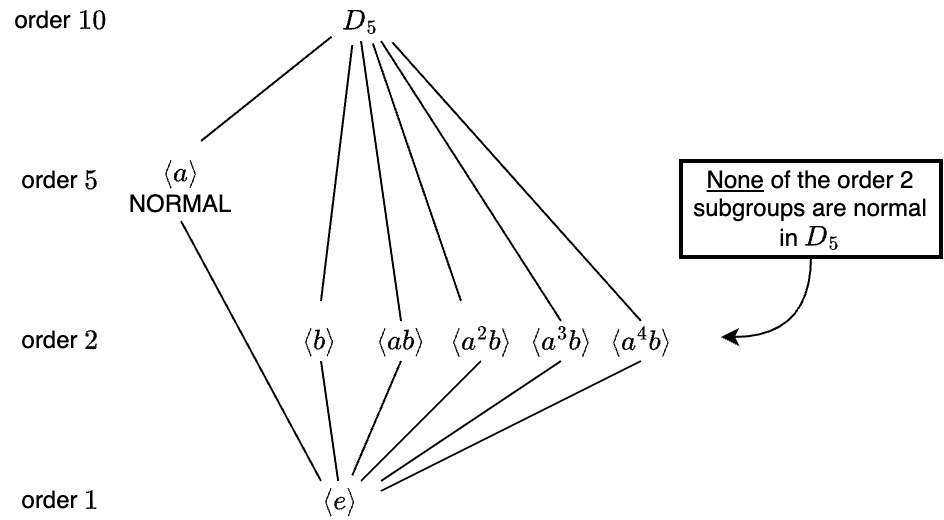
\includegraphics[width=0.85\textwidth]{Figures/HW6_Subgroup_Lattice.png}
        \end{center}
    \end{itemize}

\end{enumerate}

\newpage 



\section{Homework \# 7}
\markright{\sffamily\normalsize Homework \# 7} % manually set the section header
\label{sec:HW7}
\index{Homework 007@Homework \#7}

\begin{enumerate}
    \item Find the order and parity of \( \theta \) in the group \( S_9 \):
    \[
    \theta = (6,5,9,3,2,7)(8,6,7,9)(6,3,5)(3,2,6)(6,3)(5,8,2,9)
    \]

    \item Find the order and parity of the commutator \( [\sigma, \tau] \in S_9 \) where 
    \[
    \sigma = (1,3,7,5) \quad \text{and} \quad \tau = (2,7,8,6)(6,9,4,3).
    \]

    \item Assume \( G \) is a group with \( o(G) = 1,331 = 11^3 \) and \( o(Z(G)) = 11 \).  
    Use the class equation to determine the exact number of conjugate classes in \( G \). \\ \steezybreak

\end{enumerate}

\noindent \rule{\textwidth}{0.4pt} \\ \steezybreak

\noindent \textbf{Preliminaries for (4)--(7):}  
We know that the converse of Lagrange's Theorem is false in general. However, \textit{the converse is true for cyclic groups}, in particular, for the \( \mathbb{Z}_n \)'s.  
(Recall \( \mathbb{Z}_n = \langle 1 \rangle \) under \( + \mod n \).)  
We can even say more: in a cyclic group, not only do we get a subgroup for each divisor of the order, we get \textbf{EXACTLY ONE} subgroup for each divisor. So here is the \textbf{Theorem}:  
\begin{theorem*}[A Scenario where the converse of Lagrange holds]
    If $G$ is cyclic  of finite order, then \(\forall d \in \mathbb{Z}^+ \ni  d \mid o(G)\), there exists one and only one subgroup in $G$ of order $d$.
\end{theorem*}
\noindent Problems (4)--(6) prove this theorem; note that there are two things to prove: \textbf{existence} (\(\exists\) one) and \textbf{uniqueness} ("and only one"). \\ \steezybreak

\noindent \rule{\textwidth}{0.4pt} \\ \steezybreak

\noindent Given: \( G = \langle x \rangle \) and \( o(G) = n \).  \\
\noindent Assume \( d \in \mathbb{Z}^+ \) with \( d \mid n \). \\

\begin{enumerate}
    \setcounter{enumi}{3} % Continue numbering from previous set
    \item Show that \( G \) has a subgroup of order \( d \) by proving that \( x^{\frac{n}{d}} \) has order \( d \).  
    (Then the subgroup of order \( d \) is \( \langle x^{\frac{n}{d}} \rangle \).)  
    \mbox{}\hfill \textit{(proving existence)} \\ \steezybreak
    
    \item Define the set 
    \[
    G_d = \{ g \in G \mid g^d = e \}.
    \]
    Show that \( G_d < G \), and that \( o(G_d) \leq d \).  
    \mbox{}\hfill \textit{(set-up for proving uniqueness)} \\ \steezybreak
    
    \item Suppose \( H < G \) with \( o(H) = d \).  
    Show that \( H = \langle x^{\frac{n}{d}} \rangle \)  
    by showing that both \( H \) and \( \langle x^{\frac{n}{d}} \rangle \) are equal to \( G_d \).  
    \mbox{}\hfill \textit{(proving uniqueness)} \\ \steezybreak
    
    \item Apply the Theorem to find the subgroup lattice of \( \mathbb{Z}_{30} \).  
    \begin{itemize}
        \item Note that (4) actually gives you the generators of each subgroup.
    \end{itemize}
\end{enumerate}
\newpage 

\section{Homework \# 8}
\markright{\sffamily\normalsize Homework \# 8} % manually set the section header
\label{sec:HW8}
\index{Homework 008@Homework \#8}

\begin{enumerate}
    \item Suppose \( G \) is a group of order \( n \). Cayley’s Theorem says there must be a subgroup of \( S_n \) which is isomorphic to \( G \).  
    This ``\textit{subgroup of \( S_n \)}" is known as \( G \)'s \textit{permutation representation}.  

    Find the \textbf{GENERATORS} of the permutation representation for your personal group.  \\ \steezybreak

    \item[] \rule{\textwidth}{0.4pt} \\ \steezybreak

    In class, we’ve seen (most recently in the Sylow examples) that for \( H, K < G \), \( o(H \cap K) \) is always \textit{a common divisor} of \( o(H) \) and \( o(K) \),  
    and as such, if \( o(H) \) and \( o(K) \) happen to be \textit{relatively prime}, then  
    \( o(H \cap K) = 1 \), which in turn forces \( H \cap K = \{e\} \).  \\ \steezybreak

    Let’s name this result for convenient use in  
    \textit{“Sylow-type”} problems (like the next 3).  

    \[
    \boxed{\textbf{EASY FACT:} \quad \text{If } H, K < G \text{ with } o(H) \text{ and } o(K) \text{ relatively prime, then } H \cap K = \{e\}.}
    \]

    \item[] \rule{\textwidth}{0.4pt} \\ \steezybreak

    \item Prove that a group of order 77 is cyclic.  \\ \steezybreak

    \item Prove that a group of order 351 is not simple.  \\
    (HINT: Sometimes \( G \) is just too small to accommodate a possibility suggested by Sylow \( 3 \).)  \\ \steezybreak

    \item Assume \( G \) is a simple group of order 60.  
    Determine the \textbf{exact number} of elements of order 5 in \( G \).  \\ \steezybreak

    \item Find the 2-Sylow subgroup(s) and the 3-Sylow subgroup(s) in \( \Z_3 \times \Z_6 \).  

\end{enumerate}
\newpage 

\section{Homework \# 9}
\markright{\sffamily\normalsize Homework \# 9} % manually set the section header
\label{sec:HW9}
\index{Homework 009@Homework \#9}

\section{Homework \# 10}
\markright{\sffamily\normalsize Homework \# 10} % manually set the section header
\label{sec:HW10}
\index{Homework 010@Homework \#10}

\section{Homework \# 11}
\markright{\sffamily\normalsize Homework \# 11} % manually set the section header
\label{sec:HW11}
\index{Homework 011@Homework \#11}

\section{Homework \# 12}
\markright{\sffamily\normalsize Homework \# 12} % manually set the section header
\label{sec:HW12}
\index{Homework 012@Homework \#12}

\vspace{0.35cm}
\textit{If you're feeling generous, feel free to add the \href{https://www.dropbox.com/sh/759pwsjyc3ix0jy/AADBiIq0ZkDsvyEG6fMvSxJta/Abstract\%20Algebra\%20Homework\%20Sets?dl=0&subfolder_nav_tracking=1}{other homework problems} you have worked through so far... I will try to get them all in here eventually!}